\documentclass{article}

% Language setting
% Replace `english' with e.g. `spanish' to change the document language
\usepackage[english]{babel}

% Set page size and margins
% Replace `letterpaper' with `a4paper' for UK/EU standard size
\usepackage[letterpaper,top=2cm,bottom=2cm,left=3cm,right=3cm,marginparwidth=1.75cm]{geometry}

% Useful packages
\usepackage{amsmath}
\usepackage{graphicx}
\usepackage[colorlinks=true, allcolors=blue]{hyperref}
\usepackage{bm}
\usepackage{tikz}
\usetikzlibrary{fit, positioning}

\usepackage{cleveref}
\crefname{figure}{fig.}{fig.}
\Crefname{figure}{Fig.}{Fig.}
\crefname{equation}{eq.}{eq.}
\Crefname{equation}{Eq.}{Eq.}

\usepackage[color=magenta]{todonotes}



\title{Composition of Movement Primitives}
\author{Andrea Pierré}

\begin{document}
\maketitle

% \begin{abstract}
% Your abstract.
% \end{abstract}

\tableofcontents

\section{ProMPs}
\subsection{Recap}
From \citep{paraschos_probabilistic_2013, paraschos_using_2018}:
\begin{table}
  \centering
  \caption{Notation}
  \begin{tabular}{ll}
    \toprule
    $q_t$ & joint angle over time\\
    $\dot{q}_t$ & joint velocity over time\\
    $\bm{\tau} = \{q_t\}_{t=0\dots T}$ & trajectory\\
    $\bm{w}$ & weight vector of a single trajectory $[n \times 1]$\\
    $\phi_t$ & basis function\\
    $n$ & number of basis functions\\
    $\bm{\Phi}_t = [\phi_t, \dot{\phi_t}]$ & $n \times 2$ dimensional time-dependent basis matrix\\
    $z(t)$ & monotonically increasing phase variable\\
    $\bm{\epsilon}_y \sim \mathcal{N}(\bm{0}, \bm{\Sigma}_y)$ & zero-mean i.i.d. Gaussian noise\\
    \bottomrule
  \end{tabular}
\end{table}

\begin{equation}
  \bm{\Phi}_t =
  \begin{bmatrix}
    \phi_1 & \dot{\phi_1}\\
    \vdots & \vdots\\
    \phi_n & \dot{\phi_n}
  \end{bmatrix}
\end{equation}

\begin{gather}
\bm{y}_t = \begin{bmatrix}
       q_t \\[0.3em]
       \dot{q}_t
     \end{bmatrix} = \bm{\Phi}^{\top}_{t}\bm{w} + \bm{\epsilon}_y\\
p(\bm{\tau}|\bm{w}) = \prod_t \mathcal{N}\Big(\bm{y}_t|\bm{\Phi}^{\top}_{t}\bm{w}, \bm{\Sigma}_y \Big)\\
p(\bm{\tau};\bm{\theta}) = \int p(\bm{\tau}|\bm{w}) \cdot p(\bm{w};\bm{\theta}) d\bm{w}
\end{gather}

\subsection{Coupling between joints}

\begin{equation}
p(\bm{y}_t|\bm{w}) = \mathcal{N}\Bigg(
        \begin{bmatrix}
                \bm{y}_{1,t} \\
                \vdots\\
                \bm{y}_{d,t} \\
        \end{bmatrix}
        \Bigg|
        \begin{bmatrix}
                \bm{\Phi}^{\top}_{t} & \cdots & \bm{0} \\
                \vdots &\ddots & \vdots\\
                \bm{0} & \cdots & \bm{\Phi}^{\top}_{t} \\
        \end{bmatrix}
        \bm{w}, \bm{\Sigma}_y
\Bigg) = \mathcal{N}\Big(\bm{y}_t|\bm{\Psi}_t\bm{w},\bm{\Sigma}_y \Big)
\end{equation}

with:
\begin{table}[h]
  \centering
  \caption{Notation}
  \begin{tabular}{ll}
    \toprule
    $\bm{w}=[\bm{w}^\top_1, \dots, \bm{w}^\top_n]^\top$ & combined weight vector $[n \times n]$\\
     $\bm{\Psi}_t$ & block-diagonal basis matrix containing the basis functions and\\&their derivatives for each dimension\\
     $\bm{y}_{i,t} = [q_{i,t}, \dot{q}_{i,t}]^\top$ & joint angle and velocity for the $i^{\text{th}}$ joint\\
     \bottomrule
  \end{tabular}
\end{table}

\subsection{Hierarchical Bayesian Model}

The Hierarchical Bayesian Model used in ProMPs is illustrated in \Cref{fig:HBM}.

\begin{figure}[htbp]
\centering
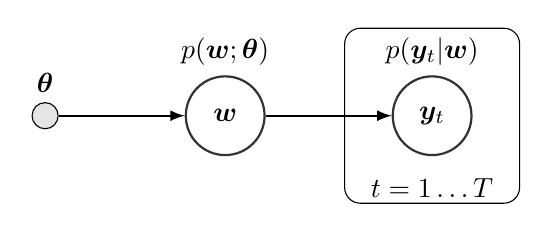
\begin{tikzpicture}
\tikzstyle{main}=[circle, minimum size = 10mm, thick, draw =black!80, node distance = 16mm]
\tikzstyle{connect}=[-latex, thick]
\tikzstyle{box}=[rectangle, draw=black!100]
  \node[circle, draw=black!100, fill = black!10] (theta) [label=above:$\bm{\theta}$] { };
  \node[main] (w) [right=of theta,label=above:$p(\bm{w};\bm{\theta})$] {$\bm{w}$};
  \node[main] (y) [right=of w,label=above:$p(\bm{y}_t|\bm{w})$] {$\bm{y}_t$};
  \path (theta) edge [connect] (w)
		(w) edge [connect] (y);
  \node[rectangle, inner sep=1.5mm, fit= (y),label=below:{$t=1 \dots T$}] (ghost) {};
  \node[rectangle, rounded corners=0.2cm, inner sep=4.4mm,draw=black!100, fit= (y) (ghost)] {};
\end{tikzpicture}
\caption{Hierarchical Bayesian Model used in ProMPs.}
\label{fig:HBM}
\end{figure}

\begin{table}
  \centering
  \caption{Notation}
  \begin{tabular}{ll}
    \toprule
    $\bm{\theta} = \{\bm{\mu}_{w}, \bm{\Sigma}_{w}\}$ & parameters\\
    $p(\bm{w};\bm{\theta}) = \mathcal{N}(\bm{w}|\bm{\mu}_{w}, \bm{\Sigma}_{w})$ & prior over the weight vector $\bm{w}$, with parameters $\bm{\theta}$, assumed to be Gaussian\\
     \bottomrule
  \end{tabular}
\end{table}

\begin{align}
p(\bm{y}_t; \bm{\theta}) &= \int \mathcal{N}\Big(\bm{y}_t|\bm{\Psi}^\top_t \bm{w}, \bm{\Sigma}_y \Big) \cdot p(\bm{w}; \bm{\theta}) \; d\bm{w}\\
&= \int \mathcal{N}\Big(\bm{y}_t|\bm{\Psi}^\top_t \bm{w}, \bm{\Sigma}_y \Big) \cdot \mathcal{N}\Big(\bm{w}|\bm{\mu_w}, \bm{\Sigma_w} \Big) \; d\bm{w}\\
&= \mathcal{N}\Big( \bm{y}_t | \bm{\Psi}^\top_t \bm{\mu_w}, \bm{\Psi}^\top_t \bm{\Sigma_w} \bm{\Psi}_t + \bm{\Sigma}_y \Big)\label{eq:HBM}
\end{align}
See \Cref{proof:HBM} for the proof.


\subsection{Via-Points Modulation}

\begin{table}
  \centering
  \caption{Notation}
  \begin{tabular}{ll}
    \toprule
    $\bm{x}_t^\star = [\bm{y}_t^\star, \bm{\Sigma}^\star_t]$ & desired observation\\
     $\bm{y}^\star_t$ & desired position and velocity vector at time $t$\\
     $\bm{\Sigma}^\star_t$ & accuracy of the desired observation\\
      \bottomrule
  \end{tabular}
\end{table}

Using Bayes rule:
\begin{align}
  p(\bm{w}|\bm{x}_t^\star) &= \frac{p(\bm{x}_t^\star|\bm{w}) \cdot p(\bm{w})}{p(\bm{x}_t^\star)} \\
  p(\bm{w}|\bm{x}_t^\star) &\propto \mathcal{N}\Big( \bm{y}_t^\star | \bm{\Psi}_t^\top\bm{w}, \bm{\Sigma}^\star_t \Big) \cdot \mathcal{N}(\bm{w}|\bm{\mu}_{w}, \bm{\Sigma}_{w})\label{eq:prob-cond-new}
\end{align}

\begin{align}
\bm{\mu_w}^{[new]} &= \bm{\mu_w} + \bm{\Sigma_w}\bm{\Psi}_t \Big(\bm{\Sigma}_y^\star + \bm{\Psi}_t^\top \bm{\Sigma_w}\bm{\Psi}_t \Big)^{-1} (\bm{y}_t^\star - \bm{\Psi}_t^\top \bm{\mu_w})\label{eq:mu-cond-new}\\
\bm{\Sigma_w}^{[new]} &= \bm{\Sigma_w} - \bm{\Sigma_w}\bm{\Psi}_t \Big(\bm{\Sigma}_y^\star +  \bm{\Psi}_t^\top \bm{\Sigma_w}\bm{\Psi}_t \Big)^{-1} \bm{\Psi}_t^\top \bm{\Sigma_w}\label{eq:sigma-cond-new}
\end{align}
See \Cref{proof:conditioning} for the proof.


\subsubsection{Do we actually get the desired mean by applying the conditioning update?}

\begin{proof}[Proof that the posterior mean equals the observed mean]
\begin{equation}
  \E[\bm{y}_{t}|\bm{x}_{t}^{\star}] = \bm{\mu}_{\bm{y}_{t}|\bm{x}_{t}^{\star}} = \textcolor[rgb]{0,0.5,1}{\bm{\Psi}_t^\top} \bm{\mu}_{\bm{w}|\bm{x}_t^\star} = \textcolor[rgb]{0,0.5,1}{\bm{\Psi}_t^\top} \bm{\mu_w} + \textcolor[rgb]{0,0.5,1}{\bm{\Psi}_t^\top} \bm{\Sigma_w}\bm{\Psi}_t \Big(\bm{\Sigma}_t^\star + \bm{\Psi}_t^\top \bm{\Sigma_w}\bm{\Psi}_t \Big)^{-1} (\bm{y}_t^\star - \bm{\Psi}_t^\top \bm{\mu_w})
                          % &\stackrel{?}{=} \bm{y}_t^\star
  \end{equation}
  We set the observed covariance $\bm{\Sigma}_t^\star$ to $0$ so as to have perfect accuracy around our observed position.
\begin{align}
  \bm{\Psi}_t^\top \bm{\mu}_{\bm{w}|\bm{x}_t^\star} &= \bm{\Psi}_t^\top \bm{\mu_w} + \cancel{\bm{\Psi}_t^\top \bm{\Sigma_w}\bm{\Psi}_t} \Big( \cancel{\bm{\Psi}_t^\top \bm{\Sigma_w}\bm{\Psi}_t} \Big)^{-1} (\bm{y}_t^\star - \bm{\Psi}_t^\top \bm{\mu_w})\\
                                   &= \cancel{\bm{\Psi}_t^\top \bm{\mu_w}} + \bm{y}_t^\star - \cancel{\bm{\Psi}_t^\top \bm{\mu_w}}\\
                                   &= \bm{y}_t^\star
  \end{align}
  \end{proof}

  \subsubsection{Multi via-points}

\begin{figure}[htbp]
  \centering
  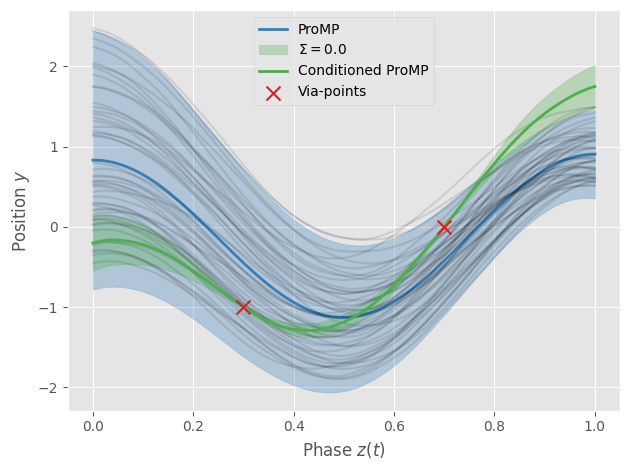
\includegraphics[width=0.5\linewidth]{fig/2-via-points.png}
  \caption{Example of ProMP with two via-points.}
  \label{fig:multi-via-pts}
\end{figure}

\begin{enumerate}
\item For the first via-point conditioning update with the observed via-point $\bm{x}_{t_{1}}^\star = [\bm{y}_{t_{1}}^\star, \bm{\Sigma}^\star_{t_{1}}]$, we can directly apply \Cref{eq:mu-cond-new,eq:sigma-cond-new}, with $\bm{\Psi}_{t_1}$ the observation matrix at time $t_{1}$:
\begin{align}
\bm{\mu}_{\bm{w}|\bm{x}_{t_{1}}^\star} &= \bm{\mu_w} + \bm{\Sigma_w}\bm{\Psi}_{t_1} \Big(\bm{\Sigma}_{t_{1}}^\star + \bm{\Psi}_{t_1}^\top \bm{\Sigma_w}\bm{\Psi}_{t_1} \Big)^{-1} (\bm{y}_{t_{1}}^\star - \bm{\Psi}_{t_1}^\top \bm{\mu_w})\\
\bm{\Sigma}_{\bm{w}|\bm{x}_{t_{1}}^\star} &= \bm{\Sigma_w} - \bm{\Sigma_w}\bm{\Psi}_{t_1} \Big(\bm{\Sigma}_{t_{1}}^\star +  \bm{\Psi}_{t_1}^\top \bm{\Sigma_w}\bm{\Psi}_{t_1} \Big)^{-1} \bm{\Psi}_{t_1}^\top \bm{\Sigma_w}
\end{align}

\item For the second via-point conditioning update with the observed via-point $\bm{x}_{t_{2}}^\star = [\bm{y}_{t_{2}}^\star, \bm{\Sigma}^\star_{t_{2}}]$, the prior is the posterior from the first via-point, \ie{} $\bm{w} \sim \mathcal{N}(\bm{\mu}_{\bm{w}|\bm{x}_{t_{1}}^\star}, \bm{\Sigma}_{\bm{w}|\bm{x}_{t_{1}}^\star})$, the likelihood is $\bm{y}_{t_{2}}^\star \sim \mathcal{N}(\bm{\Psi}_{t_2}^\top \bm{w}, \bm{\Sigma}_{t_{2}}^\star)$, with $\bm{\Psi}_{t_2}$ the observation matrix at time $t_{2}$, and the posterior update becomes:
\begin{align}
\bm{\mu}_{\bm{w}|\bm{x}_{t_{1}}^{\star}, \bm{x}_{t_{2}}^\star} &= \bm{\mu}_{\bm{w}|\bm{x}_{t_{1}}^\star} + \bm{\Sigma}_{\bm{w}|\bm{x}_{t_{1}}^\star}\bm{\Psi}_{t_2} \Big(\bm{\Sigma}_{t_{2}}^\star + \bm{\Psi}_{t_2}^\top \bm{\Sigma}_{\bm{w}|\bm{x}_{t_{1}}^\star}\bm{\Psi}_{t_2} \Big)^{-1} (\bm{y}_{t_{2}}^\star - \bm{\Psi}_{t_2}^\top \bm{\mu}_{\bm{w}|\bm{x}_{t_{1}}^\star})\\
\bm{\Sigma}_{\bm{w}|\bm{x}_{t_{1}}^{\star}, \bm{x}_{t_{2}}^\star} &= \bm{\Sigma}_{\bm{w}|\bm{x}_{t_{1}}^\star} - \bm{\Sigma}_{\bm{w}|\bm{x}_{t_{1}}^\star}\bm{\Psi}_{t_2} \Big(\bm{\Sigma}_{t_{2}}^\star +  \bm{\Psi}_{t_2}^\top \bm{\Sigma}_{\bm{w}|\bm{x}_{t_{1}}^\star}\bm{\Psi}_{t_2} \Big)^{-1} \bm{\Psi}_{t_2}^\top \bm{\Sigma}_{\bm{w}|\bm{x}_{t_{1}}^\star}
\end{align}

\item For the $k^{\text{th}}$ via-point conditioning update with the observed via-point $\bm{x}_{t_{k}}^\star = [\bm{y}_{t_{k}}^\star, \bm{\Sigma}^\star_{t_{k}}]$, the prior is the posterior after conditioning on the previous $k-1$ via-points, \ie{} $\bm{w} \sim \mathcal{N}(\bm{\mu}_{\bm{w}|\bm{x}_{t_{1}}^\star, \dots, \bm{x}_{t_{k-1}}^\star}, \allowbreak \bm{\Sigma}_{\bm{w}|\bm{x}_{t_{1}}^\star, \dots, \bm{x}_{t_{k-1}}^\star})$, the likelihood is $\bm{y}_{t_{k}}^\star \sim \mathcal{N}(\bm{\Psi}_{t_k}^\top \bm{w}, \bm{\Sigma}_{t_{k}}^\star)$, with $\bm{\Psi}_{t_k}$ the observation matrix at time $t_{k}$, and the posterior update becomes:
\begin{align}
\begin{split}
\bm{\mu}_{\bm{w}|\bm{x}_{t_{1}}^\star, \dots, \bm{x}_{t_{k}}^\star} &= \bm{\mu}_{\bm{w}|\bm{x}_{t_{1}}^\star, \dots, \bm{x}_{t_{k-1}}^\star} \\&\quad+ \bm{\Sigma}_{\bm{w}|\bm{x}_{t_{1}}^\star, \dots, \bm{x}_{t_{k-1}}^\star}\bm{\Psi}_{t_k} \Big(\bm{\Sigma}_{t_{k}}^\star + \bm{\Psi}_{t_k}^\top \bm{\Sigma}_{\bm{w}|\bm{x}_{t_{1}}^\star, \dots, \bm{x}_{t_{k-1}}^\star}\bm{\Psi}_{t_k} \Big)^{-1} (\bm{y}_{t_{k}}^\star - \bm{\Psi}_{t_k}^\top \bm{\mu}_{\bm{w}|\bm{x}_{t_{1}}^\star, \dots, \bm{x}_{t_{k-1}}^\star})
\end{split}\\
\begin{split}
\bm{\Sigma}_{\bm{w}|\bm{x}_{t_{1}}^\star, \dots, \bm{x}_{t_{k}}^\star} &= \bm{\Sigma}_{\bm{w}|\bm{x}_{t_{1}}^\star, \dots, \bm{x}_{t_{k-1}}^\star} \\&\quad- \bm{\Sigma}_{\bm{w}|\bm{x}_{t_{1}}^\star, \dots, \bm{x}_{t_{k-1}}^\star}\bm{\Psi}_{t_k} \Big(\bm{\Sigma}_{t_{k}}^\star +  \bm{\Psi}_{t_k}^\top \bm{\Sigma}_{\bm{w}|\bm{x}_{t_{1}}^\star, \dots, \bm{x}_{t_{k-1}}^\star}\bm{\Psi}_{t_k} \Big)^{-1} \bm{\Psi}_{t_k}^\top \bm{\Sigma}_{\bm{w}|\bm{x}_{t_{1}}^\star, \dots, \bm{x}_{t_{k-1}}^\star}
\end{split}
\end{align}
\end{enumerate}

\paragraph{Alternative Batch Formulation}
Instead of iterative updates, we could condition on all via-points simultaneously by stacking the observations:
\begin{equation}
  \bm{y}^{\star} =
  \begin{bmatrix}
    \bm{y}^{\star}_{t_{1}}\\
    \vdots \\
    \bm{y}^{\star}_{t_{k}}
  \end{bmatrix}, \quad
  \bm{\Psi} =
  \begin{bmatrix}
    \bm{\Psi}_{t_{1}}\\
    \vdots \\
    \bm{\Psi}_{t_{k}}
  \end{bmatrix}, \quad
  \bm{\Sigma}^\star = \diag(\bm{\Sigma}^\star_{t_{1}}, \dots, \bm{\Sigma}^\star_{t_{k}})
\end{equation}

\begin{align}
\bm{\mu}_{\bm{w}|\{\bm{x}_{t_k}^\star\}_{k=1}^K} &= \bm{\mu_w} + \bm{\Sigma_w}\bm{\Psi} \Big(\bm{\Sigma}^\star + \bm{\Psi}^\top \bm{\Sigma_w}\bm{\Psi} \Big)^{-1} (\bm{y}^\star - \bm{\Psi}^\top \bm{\mu_w})\\
\bm{\Sigma}_{\bm{w}|\{\bm{x}_{t_k}^\star\}_{k=1}^K} &= \bm{\Sigma_w} - \bm{\Sigma_w}\bm{\Psi} \Big(\bm{\Sigma}^\star + \bm{\Psi}^\top \bm{\Sigma_w}\bm{\Psi} \Big)^{-1} \bm{\Psi}^\top \bm{\Sigma_w}
\end{align}


\section{Gaussian mixture modeling (GMM)/Gaussian mixture regression (GMR) recap}
\subsection{Gaussian Mixture Modeling (GMM)}
\begin{table}
  \centering
  \caption{Notation}
  \begin{tabular}{ll}
    \toprule
    $\pi_{k}$ & mixture weights\\
     $\bm{\theta} := \{\bm{\mu}_{k}, \bm{\Sigma}_{k}, \pi_{k}: k=1, \dots, K\}$ & collection of all parameters of the model\\
     $r_{nk}$ & responsibility of the $k^{\text{th}}$ mixture component for the $n^{\text{th}}$ data point\\
     $N$ & number of data points\\
     $N_{k} := \sum^{N}_{n=1} r_{nk}$ & total responsibility of the $k^{\text{th}}$ mixture component for the entire dataset\\
       \bottomrule
  \end{tabular}
\end{table}

\begin{gather}
  p(\bm{x}|\bm{\theta}) = \sum^{K}_{k=1} \pi_{k}  \mathcal{N}(\bm{x}|\bm{\mu}_{k}, \bm{\Sigma}_{k})\\
  0 \leq \pi_{k} \leq 1, \quad \sum^{K}_{k=1} \pi_{k} = 1\\
  r_{nk} := \frac{\pi_{k}  \mathcal{N}(\bm{x}_{n}|\bm{\mu}_{k}, \bm{\Sigma}_{k})}{\sum^{K}_{j=1} \pi_{j}  \mathcal{N}(\bm{x}_{n}|\bm{\mu}_{j}, \bm{\Sigma}_{j})}
\end{gather}
Update of the GMM means:
\begin{equation}
  \bm{\mu}_{k}^{new} = \frac{\sum_{n=1}^{N}r_{nk}\bm{x}_{n}}{\sum_{n=1}^{N}r_{nk}}
\end{equation}
Update of the GMM covariances:
\begin{equation}
  \bm{\Sigma}_{k}^{new} = \frac{1}{N_{k}} \sum^{N}_{n=1} r_{nk} (\bm{x}_{n} - \bm{\mu}_{k})(\bm{x}_{n} - \bm{\mu}_{k})^{\top}
\end{equation}
Update of the GMM mixture weights:
\begin{equation}
  \pi_{k}^{new} = \frac{N_{k}}{N}, \quad k=1, \dots, K
\end{equation}

The parameters are updated using \Cref{algo:EM}.


\begin{algorithm}[htbp]
\caption{\textsc{Expectation Maximization (EM)} algorithm for a Gaussian mixture model}
\label{algo:EM}
\DontPrintSemicolon
\SetKwInOut{Input}{Input}
\SetKwInOut{Output}{Output}
\SetKwFunction{KwPrint}{Print}
\SetKwProg{Func}{Function}{}{end}
\SetKw{KwLet}{let}

\Input{Initial model parameters $\{\bm{\mu}_{k}\}$, $\{\bm{\Sigma}_{k}\}$, $\{\pi_{k}\}$}
\Input{Data set $\{\bm{\mathrm{x}}_{1}, \dots, \bm{\mathrm{x}}_{N}\}$}
\Output{Final model parameters $\{\bm{\mu}_{k}\}$, $\{\bm{\Sigma}_{k}\}$, $\{\pi_{k}\}$}
\BlankLine

\Repeat{convergence}{
  \BlankLine
  \tcp{E-step}
  \For{$n \in \{1, \dots, N\}$}{
    \For{$k \in \{1, \dots, K\}$}{
      \begin{flalign*}
        &r_{nk} \gets \frac{\pi_{k}  \mathcal{N}(\bm{\mathrm{x}}_{n}|\bm{\mu}_{k}, \bm{\Sigma}_{k})}{\sum^{K}_{j=1} \pi_{j}  \mathcal{N}(\bm{\mathrm{x}}_{n}|\bm{\mu}_{j}, \bm{\Sigma}_{j})}&
      \end{flalign*}
    }
  }

  \BlankLine
  \tcp{M-step}
  \For{$k \in \{1, \dots, K\}$}{
      \begin{flalign*}
        N_{k} &= \sum_{n=1}^{N}r_{nk}&\\
        \bm{\mu}_{k} &= \frac{1}{N_{k}} \sum_{n=1}^{N}r_{nk}\bm{\mathrm{x}}_{n}&\\
        \bm{\Sigma}_{k} &= \frac{1}{N_{k}} \sum^{N}_{n=1} r_{nk} (\bm{\mathrm{x}}_{n} - \bm{\mu}_{k})(\bm{\mathrm{x}}_{n} - \bm{\mu}_{k})^{\top}&\\
        \pi_{k} &= \frac{N_{k}}{N}&
      \end{flalign*}
  }

  \BlankLine
  \tcp{Log likelihood}%
  \vspace{-1.5em}
      \begin{flalign*}%
        &\mathcal{L} \gets \sum^{N}_{n=1} \ln \Bigg\{\sum^{K}_{k=1} \pi_{k}  \mathcal{N}(\bm{\mathrm{x}}_{n}|\bm{\mu}_{k}, \bm{\Sigma}_{k}) \Bigg\}&
      \end{flalign*}
}
\Return{$\{\bm{\mu}_{k}\}$, $\{\bm{\Sigma}_{k}\}$, $\{\pi_{k}\}$}
\end{algorithm}

\subsection{Gaussian Mixture Regression (GMR)}

At each iteration step $t$, the datapoint $\bm{x}_{t}$ can be decomposed as two subvectors $\bm{x}_{t}^{I}$ and $\bm{x}_{t}^{O}$ spanning for the input and output dimensions. For trajectory encoding in task space, $I$ corresponds to the time input dimension (\eg value of a decay term), and $O$ corresponds to the output dimensions describing a path (\eg end-effector position in task space).

During the training phase we learn the joint probability $p(\bm{x}_{t}^{I}, \bm{x}_{t}^{O})$ with GMM through EM (\Cref{algo:EM}) with:
\begin{table}[h]
  \centering
  \caption{Notation}
  \begin{tabular}{ll}
    \toprule
    $\bm{x}_{t} \in \mathbb{R}^{D}$ & datapoint at timestep $t$\\
    $\bm{\mu}_{k}$ & center of the $k^{\text{th}}$ Gaussian\\
    $\bm{\Sigma}_{k}$ & covariance of the $k^{\text{th}}$ Gaussian\\
    \bottomrule
  \end{tabular}
\end{table}

\begin{align}
  p(\bm{x}_{t}^{I}, \bm{x}_{t}^{O}) &=  \sum_{k=1}^{K}\pi_{k} \mathcal{N}_{k}(\bm{x}_{t}^{I}, \bm{x}_{t}^{O}|\bm{\mu}_{k}, \bm{\Sigma}_{k})\\
  % &= \sum^{K}_{i=1} \pi_{i} \cdot \mathcal{N}_{i}(x_{j}|t_{j};m_{i}(t_{j}),cov_{i}) \cdot \mathcal{N}_{i}(t_{j}|\bm{\mu}_{it}, \bm{\Sigma}_{it})\\
  &=  \sum_{k=1}^{K}\pi_{k} p(\bm{x}_{t}^{O}|\bm{x}_{t}^{I}) \cdot p(\bm{x}_{t}^{I})\\
  &=  \sum_{k=1}^{K}\pi_{k} \mathcal{N}_{k}(\hat{\bm{\mu}}_{k}^{O}(\bm{\mu}_{k}^{I}), \hat{\bm{\Sigma}}_{k}^{O}) \cdot \mathcal{N}_{k}(\bm{\mu}_{k}^{I}, \bm{\Sigma}_{k}^{I})
\end{align}

\begin{gather}
  \bm{x}_{t} =
  \begin{bmatrix}
    \bm{x}_{t}^{I} \\[0.5em]
    \bm{x}_{t}^{O}
  \end{bmatrix}, \quad
  \bm{\mu}_{k} =
  \begin{bmatrix}
    \bm{\mu}_{k}^{I} \\[0.5em]
    \bm{\mu}_{k}^{O}
  \end{bmatrix}, \quad
  \bm{\Sigma}_{k} =
  \begin{bmatrix}
    \bm{\Sigma}_{k}^{I} & \bm{\Sigma}_{k}^{IO}\\[0.5em]
    \bm{\Sigma}_{k}^{OI} & \bm{\Sigma}_{k}^{O}
  \end{bmatrix}\\
\end{gather}
\begin{align}
  \hat{\bm{\mu}}_{k}^{O}(\bm{x}_{t}^{I}) &= \bm{\mu}_{k}^{O} + \bm{\Sigma}_{k}^{OI}  {\bm{\Sigma}_{k}^{I}}^{-1}  (\bm{x}_{t}^{I} - \bm{\mu}_{k}^{I})\\
  \hat{\bm{\Sigma}}_{k}^{O} &= \bm{\Sigma}_{k}^{O} - \bm{\Sigma}_{k}^{OI}  {\bm{\Sigma}_{k}^{I}}^{-1} \cdot \bm{\Sigma}_{k}^{IO}
\end{align}

The marginal probability $p(\bm{x}_{t}^{I})$ is:
\begin{equation}
  p(\bm{x}_{t}^{I}) = \int p(\bm{x}_{t}^{I}, \bm{x}_{t}^{O})d\bm{x}_{t}^{O} = \sum_{k=1}^{K} \pi_{k} \cdot \mathcal{N}_{k}(\bm{\mu}_{k}^{I}, \bm{\Sigma}_{k}^{I})
\end{equation}

To retrieve the multimodal conditional distribution $p(\bm{x}_{t}^{O}|\bm{x}_{t}^{I})$ for each input/timestep we have:
\begin{align}
  p(\bm{x}_{t}^{O}|\bm{x}_{t}^{I}) &= \frac{p(\bm{x}_{t}^{O},\bm{x}_{t}^{I})}{p(\bm{x}_{t}^{I})}\\
  &= \frac{\sum_{k=1}^{K}\textcolor[rgb]{0,0.5,1}{\pi_{k}} \mathcal{N}_{k}(\hat{\bm{\mu}}_{k}^{O}(\bm{\mu}_{k}^{I}), \hat{\bm{\Sigma}}_{k}^{O}) \cdot \textcolor[rgb]{0,0.5,1}{\mathcal{N}_{k}(\bm{\mu}_{k}^{I}, \bm{\Sigma}_{k}^{I})}}{\textcolor[rgb]{0,0.5,1}{\sum_{k=1}^{K} \pi_{i} \cdot \mathcal{N}_{k}(\bm{\mu}_{k}^{I}, \bm{\Sigma}_{k}^{I})}}\\
  &= \sum_{k=1}^{K} \textcolor[rgb]{0,0.5,1}{r_{nk}} \cdot \mathcal{N}_{k}(\hat{\bm{\mu}}_{k}^{O}(\bm{\mu}_{k}^{I}), \hat{\bm{\Sigma}}_{k}^{O})
\end{align}

When a unimodal output distribution is required, the law of total mean and variance can be used to approximate the distribution with the Gaussian (see \Cref{proof:approx-multimod-to-single}):
\todo[inline]{ToDo}
\begin{align}
  m(x) &= \E(x_{j}|t_{j}) = \sum_{i=1}^{K} r_{nk} \cdot m_{i}(t_{j})\label{eq:GMR:mean}\\
  var(x) &= \sum_{j=1}^{K} r_{nk} \cdot cov_{i}\label{eq:GMR:var}
\end{align}


\section{Composition of MPs}
\subsection{Stitching}
The main issue with stitching is the smoothness of the mean and covariance between ProMPs, see \Cref{fig:stitching}.
\begin{figure}[htbp]
  \centering
  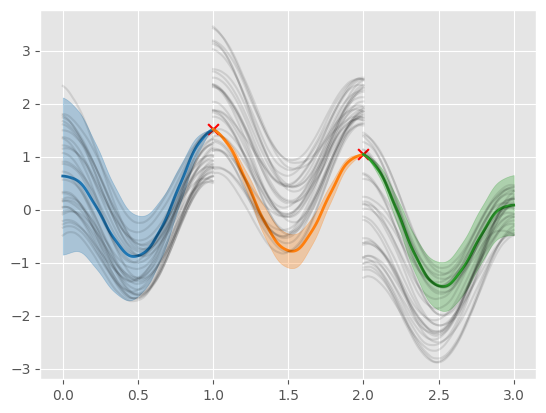
\includegraphics[width=0.5\linewidth]{fig/stitching.png}
  \caption{Stitching three ProMPs.}
  \label{fig:stitching}
\end{figure}

\subsection{Piecewise Gaussian Process}


% \newpage
\FloatBarrier
\bibliographystyle{IEEEtranN}
\bibliography{references}


\appendix
\section{Hierarchical Bayesian Model proof}

\begin{proof}[Proof of \Cref{eq:HBM}]\label{proof:HBM}
From \citep{deisenroth2020mathematics}, we have the joint distribution:
\begin{equation}
  p(\bm{\mathrm{x}}_{a}, \bm{\mathrm{x}}_{b}) = \mathcal{N}\Bigg(
  \begin{bmatrix}
    \bm{\mu}_{a} \\
    \bm{\mu}_{b} \\
  \end{bmatrix},
  \begin{bmatrix}
    \bm{\Sigma}_{aa} & \bm{\Sigma}_{ab}  \\
    \bm{\Sigma}_{ba} & \bm{\Sigma}_{bb}
  \end{bmatrix}
  \Bigg)\label{eq:joint-distrib}
\end{equation}

and the marginal distribution $p(\bm{\mathrm{x}}_{a})$ of a joint Gaussian distribution $p(\bm{\mathrm{x}}_{a}, \bm{\mathrm{x}}_{b})$:
\begin{equation}
  p(\bm{\mathrm{x}}_{a}) = \int p(\bm{\mathrm{x}}_{a}, \bm{\mathrm{x}}_{b}) d \bm{\mathrm{x}}_{b} = \mathcal{N}( \bm{\mathrm{x}}_{a} | \bm{\mu}_{a}, \bm{\Sigma}_{aa})
\end{equation}

Since $\bm{y}_t$ and $\bm{w}$ are jointly Gaussian, we have:
\begin{equation}
  \begin{bmatrix}
    \bm{y}_t \\
    \bm{w}
  \end{bmatrix} \sim \mathcal{N}\Bigg(
  \begin{bmatrix}
    \bm{\mu}_{\bm{y}_{t}} \\
    \bm{\mu_w} \\
  \end{bmatrix},
  \begin{bmatrix}
    \mathrm{Cov}[\bm{y}_t, \bm{y}_t] & \mathrm{Cov}[\bm{y}_t, \bm{w}]  \\
    \mathrm{Cov}[\bm{w}, \bm{y}_t] & \mathrm{Cov}[\bm{w}, \bm{w}]
  \end{bmatrix}
  \Bigg)
\end{equation}
\begin{align}
  \bm{\mu}_{\bm{y}_{t}} &= \E[\bm{y}_{t}]\\
                        &= \E[\bm{\Psi}^\top_t \bm{w} + \bm{\epsilon}_y]\\
                        &= \bm{\Psi}^\top_t \E[\bm{w}] + \E[\bm{\epsilon}_y]\\
                        &= \bm{\Psi}^\top_t \bm{\mu_w} + 0\\
                        &= \bm{\Psi}^\top_t \bm{\mu_w}
\end{align}
\begin{align}
  \mathrm{Cov}[\bm{y}_t, \bm{y}_t] &= \mathrm{Cov}[\bm{\Psi}^\top_t \bm{w} + \bm{\epsilon}_y]\\
  &= \mathrm{Cov}[\bm{\Psi}^\top_t \bm{w}] + \mathrm{Cov}[\bm{\epsilon}_y]\\
  &= \bm{\Psi}^\top_t\mathrm{Cov}[\bm{w}]\bm{\Psi}_t + \bm{\Sigma}_{y}\\
    &= \bm{\Psi}^\top_t\bm{\Sigma_{w}}\bm{\Psi}_t + \bm{\Sigma}_{y}\label{eq:cov_y_y}
\end{align}

\begin{equation}
  \begin{bmatrix}
    \bm{y}_t \\
    \bm{w}
  \end{bmatrix} \sim \mathcal{N}\Bigg(
  \begin{bmatrix}
    \bm{\Psi}^\top_t \bm{\mu_w} \\
    \bm{\mu_w} \\
  \end{bmatrix},
  \begin{bmatrix}
    \bm{\Psi}^\top_t \bm{\Sigma_w} \bm{\Psi}_t + \bm{\Sigma}_y & \bm{\Psi}^\top_t \bm{\Sigma_w}  \\
    \bm{\Sigma_w} \bm{\Psi}_t & \bm{\Sigma_w}
  \end{bmatrix}
  \Bigg)
\end{equation}
\begin{equation}
p(\bm{y}_t; \bm{\theta}) = \mathcal{N}\Big( \bm{y}_t | \bm{\Psi}^\top_t \bm{\mu_w}, \bm{\Psi}^\top_t \bm{\Sigma_w} \bm{\Psi}_t + \bm{\Sigma}_y \Big)
\end{equation}

\end{proof}

\section{Via-Points conditioning proof}

\begin{proof}[Proof of \Cref{eq:mu-cond-new} and \Cref{eq:sigma-cond-new}]\label{proof:conditioning}
  With the joint distribution $p(\bm{\mathrm{x}}_{a}, \bm{\mathrm{x}}_{b})$ in \Cref{eq:joint-distrib}, and from \citep{bishop2024learning}, the parameters of a conditional multivariate Gaussian $p(\bm{\mathrm{x}}_{a}|\bm{\mathrm{x}}_{b}) = \mathcal{N}\big( \bm{\mu}_{a|b}, \bm{\Sigma}_{a|b} \big)$ are the following:
\begin{align}
  \bm{\mu}_{a|b} &= \bm{\mu}_{a} + \bm{\Sigma}_{ab}\bm{\Sigma}_{bb}^{-1}(\bm{\mathrm{x}}_{b} - \bm{\mu}_{b})\label{eq:cond-multi-gauss-mu}\\
  \bm{\Sigma}_{a|b} &= \bm{\Sigma}_{aa} - \bm{\Sigma}_{ab}\bm{\Sigma}_{bb}^{-1}\bm{\Sigma}_{ba}\label{eq:cond-multi-gauss-sigma}
\end{align}

We want the posterior $p(\bm{w}|\bm{x}_t^\star)$, knowing the likelihood $\bm{x}_t^\star|\bm{w} \sim \mathcal{N}\Big( \bm{y}_t^\star | \bm{\Psi}_t^\top\bm{w}, \bm{\Sigma}^\star_t \Big)$, and the prior $\bm{w} \sim \mathcal{N}(\bm{w}|\bm{\mu}_{w}, \bm{\Sigma}_{w})$.

\begin{equation}
  \begin{bmatrix}
    \bm{w} \\
    \bm{x}_t^{\star}
  \end{bmatrix} \sim \mathcal{N}\Bigg(
  \begin{bmatrix}
    \bm{\mu_w} \\
    \bm{\Psi}^\top_t \bm{\mu_w}\\
  \end{bmatrix},
  \begin{bmatrix}
    \mathrm{Cov}[\bm{w}, \bm{w}] &  \mathrm{Cov}[\bm{w}, \bm{x}_t^{\star}] \\
    \mathrm{Cov}[\bm{x}_t^{\star}, \bm{w}] & \mathrm{Cov}[\bm{x}_t^{\star}, \bm{x}_t^{\star}]
  \end{bmatrix}
  \Bigg)
\end{equation}

$\mathrm{Cov}[\bm{x}_t^{\star}, \bm{x}_t^{\star}]$ follows from \Cref{eq:cov_y_y}.

\begin{align}
  \mathrm{Cov}[\bm{w}, \bm{x}_t^{\star}] &= \mathrm{Cov}[\bm{w}, \bm{\Psi}^\top_t\bm{w} + \bm{\epsilon}_y]\\
                                         &= \mathrm{Cov}[\bm{w}, \bm{\Psi}^\top_t\bm{w}] & ( \mathrm{Cov}[\bm{w}, \bm{\epsilon_y}] = 0 \text{ since } \bm{\epsilon_y} \text{ is independent of } \bm{w})\\
                                         &= \E[(\bm{w} - \bm{\mu_{w}})(\bm{\Psi}^\top_t\bm{w} - \bm{\Psi}^\top_t\bm{\mu_{w}})^{\top}]\\
                                         &= \E[(\bm{w} - \bm{\mu_{w}})(\bm{w} - \bm{\mu_{w}})^{\top}\bm{\Psi}_t]\\
                                         &= \mathrm{Cov}[\bm{w}, \bm{w}] \cdot \bm{\Psi}_t\\
                                         &= \bm{\Sigma_{w}} \bm{\Psi}_t
\end{align}

\begin{equation}
  \begin{bmatrix}
    \bm{w} \\
    \bm{x}_t^{\star}
  \end{bmatrix} \sim \mathcal{N}\Bigg(
  \begin{bmatrix}
    \bm{\mu_w} \\
    \bm{\Psi}^\top_t \bm{\mu_w}\\
  \end{bmatrix},
  \begin{bmatrix}
     \bm{\Sigma_w} & \bm{\Sigma_{w}} \bm{\Psi}_t  \\
    \bm{\Psi}^\top_t\bm{\Sigma_w} & \bm{\Psi}^\top_t \bm{\Sigma_w} \bm{\Psi}_t + \bm{\Sigma}^\star_t
  \end{bmatrix}
  \Bigg)
\end{equation}

Using \Cref{eq:cond-multi-gauss-mu} we get:
\begin{equation}
\bm{\mu}_{\bm{w}|\bm{x}_t^\star} = \bm{\mu_w} + \bm{\Sigma_w}\bm{\Psi}_t \Big(\bm{\Sigma}_t^\star + \bm{\Psi}_t^\top \bm{\Sigma_w}\bm{\Psi}_t \Big)^{-1} (\bm{y}_t^\star - \bm{\Psi}_t^\top \bm{\mu_w})
\end{equation}

Using \Cref{eq:cond-multi-gauss-sigma} we get:
\begin{equation}
\bm{\Sigma}_{\bm{w}|\bm{x}_t^\star} = \bm{\Sigma_w} - \bm{\Sigma_w}\bm{\Psi}_t \Big(\bm{\Sigma}_t^\star +  \bm{\Psi}_t^\top \bm{\Sigma_w}\bm{\Psi}_t \Big)^{-1} \bm{\Psi}_t^\top \bm{\Sigma_w}
\end{equation}
\end{proof}


\end{document}
